%%%%%%%%%%%%%%%%%%%%%%%%%%%%%%%%%%%%%%%%%
% Chair of Cyber-Physical-Systems
% Univ.-Prof. Dr. Elmar Rueckert
% Montanuniversität Leoben, Austria
% Latest Update: March 2023
%
% Disclaimer: The materials and source code are for personal use only. The material 
\documentclass[aspectratio=169]{beamer}
\usetheme{Boadilla}



\usepackage[utf8]{inputenc}       % Codificação de entrada
\usepackage[T1]{fontenc}          % Codificação de saída
\usepackage[portuguese]{babel}   % Idioma
\usepackage{XCharter}             % Fonte principal

\usepackage{qrcode}


\AtBeginDocument{\fontsize{12}{12}\selectfont}

%\usepackage{geometry}
%\geometry{papersize={210mm,150mm}}

\usepackage{color}
\usepackage{graphicx}
\usepackage{amsmath, amssymb, amsfonts}
\usepackage{bm}
\usepackage{booktabs}
\usepackage{multirow}
\usepackage{caption}
\usepackage{subfigure}
\usepackage{wrapfig}
\usepackage{multicol}
\usepackage{sidecap}
\usepackage{tikz}
\usepackage{listings}
\usepackage{siunitx}
\usepackage{pdfpages}
\usepackage{float}
\usepackage{hyperref}
\usepackage{academicons}
\usepackage{setspace}

\newcommand{\eng}[1]{\textsl{#1}}
\newcommand{\cod}[1]{\texttt{#1}}
\title[Aceleradores de Redes Neurais em FPGA]{Projetando Aceleradores de Redes Neurais em FPGA} %note that the optional arg in '[]' are displayed in the left column throughout the complete presentation
% adapt accordingly
% e.g., M.Sc. Intermediate Thesis Report
% or     B.Sc. Intermediate Thesis Report


\author[Prof. Dr. Oscar Eduardo Anacona Mosquera]{Prof. Dr. Oscar Eduardo Anacona Mosquera \newline\newline 
\scriptsize{oscar.mosquera@ufmt.br}
}%note that the optional arg in '[]' are displayed in the left column throughout the complete presentation



\AtBeginSection[]
{
	\begin{frame}{Conteúdo}
		\tableofcontents[currentsection]
	\end{frame}
}



%----------------------------------------------------------------------------------------
%	DOCUMENT
%----------------------------------------------------------------------------------------
\begin{document}
%----------------------------------------------------------------------------------------
%	TITLE PAGE
%----------------------------------------------------------------------------------------
%DO NOT CHANGE THIS FIRST SLIDE 
\begin{frame}[plain]
\titlepage
%\vspace{3cm}
%\begin{center} \color{MULTurquoise} {Chair of Cyber-Physical-Systems}\end{center}

\end{frame}


\section{Agradecimentos}



\begin{frame}{Agradecimentos}
	
	\begin{itemize}
		\item Universidade Federal de Mato Grosso (UFMT)
		\item Faculdade de Engenharia do Campus de Várzea Grande (FAENG)
		\item Instituto de Computação (IC-UFMT)
		\item Curso da Engenharia da Computação
		\item Prof. Dr. Carlos Humberto Llanos (QEPD), Professor Associado do Departamento de Engenharia Mecânica (ENM) da Universidade de Brasília (UnB)
		\item  Intel Altera
		%\item  O técnico Igor
		\item  Colaboradores
	\end{itemize}	
	
\end{frame}
%----------------------------------------------------------------------------------------
\section{Objetivos}
%----------------------------------------------------------------------------------------

\begin{frame}{Objetivos}
	Este minicurso tem como foco mostrar o caminho completo, desde o código VHDL básico até a criação de um neurônio artificial dentro de uma FPGA.
	
	\begin{itemize}
		\item \textbf{Dominar a base do VHDL:} Aprender a descrever hardware e simular antes de testar na placa.
		\item \textbf{Fluxo de Trabalho:} Configurar o Quartus II e o ModelSim para trabalharem juntos.
		\item \textbf{Entender Redes Neurais:} Conhecer a estrutura de camadas e como um neurônio toma decisões.
		\item \textbf{Unir Python e Hardware:} Treinar uma lógica em Python e usar um gerador para transformar isso em hardware real (VHDL).
		\item \textbf{Mão na Massa:} Programar a placa DE0-Nano e ver o acelerador funcionando.
	\end{itemize}
\end{frame}










%----------------------------------------------------------------------------------------
\section{Apresentação}
%----------------------------------------------------------------------------------------
\begin{frame}
	
	\frametitle{Apresentação}
	\begin{itemize}
		\justifying
		%\setbeamertemplate{itemize item}[triangle]
		\item \textbf{Nome:} Prof. Dr. Oscar Eduardo Anacona Mosquera
		\item \textbf{Formação:} Doutor e Mestre em Sistemas Mecatrônicos pela Universidade de Brasília (UnB), Bacharel em Engenharia Física pela Universidad del Cauca (Colômbia).
		\item \textbf{Áreas de Atuação:} Sistemas embarcados, Automação, Robótica, e Algoritmos de otimização.
		\begin{itemize}
			\item FPGAs, microcontroladores (PIC e Atmega) e CLPs.
		\end{itemize}
		
		\item \textbf{Professor da UFMT do curso da Engenharia da Computação da FAENG-VG.}

		\item \textbf{GitHub:} oscar-ufmt
		\item \textbf{CV Lattes:} \url{https://lattes.cnpq.br/4776138897349156}
	\end{itemize}
\end{frame}
%----------------------------------------------------------------------------------------



\begin{frame}{Acesse o Repositório do Projeto}
	\centering
	\textbf{Escaneie o código abaixo para acessar o código no GitHub:} \\
	\vspace{0.5cm}
	
	% Gera o QR Code linkando para o seu repositório
	\qrcode[height=4cm]{https://github.com/oscar-ufmt/sematec_2026}
	
	\vspace{0.5cm}
	\url{https://github.com/oscar-ufmt/sematec_2026}
\end{frame}


\section{Ementa do minicurso}
%====================================================================================================
\begin{frame}{Dia 1: Fundamentos e Prática com VHDL}
	\textbf{Conteúdo Teórico e Prático (4 Horas)}
	
	\begin{enumerate}
		\item \textbf{Introdução ao VHDL e ModelSim:} Como descrever circuitos e verificar se estão corretos via simulação.
		\item \textbf{Os 4 Experimentos Base:}
		\begin{itemize}
			\item Porta AND (Lógica básica).
			\item Sistemas Numéricos (Como o hardware entende números).
			\item Flip-Flop (Memória e sincronismo).
			\item Contador de 32 bits (Divisão de clock para ver o resultado na placa).
		\end{itemize}
		\item \textbf{Simulação com Testbench:} Criar arquivos de teste para o ModelSim.
		\item \textbf{Configuração de Hardware:} Preparar o Quartus para a placa DE0-Nano.
	\end{enumerate}
\end{frame}



\begin{frame}{Dia 2: Redes Neurais e Aceleração em FPGA}
	\textbf{Da Teoria ao Neurônio no Hardware (4 Horas)}
	
	\begin{enumerate}
		\item \textbf{Introdução às Redes Neurais:} O que são camadas, pesos e funções de ativação.
		\item \textbf{Treinamento em Python:}
		\begin{itemize}
			\item Uso da biblioteca \textit{xx} para treinar portas lógicas (OR, AND, XOR).
			\item Entendendo os resultados do treinamento.
		\end{itemize}
		\item \textbf{Gerador de Redes Neurais:}
		\begin{itemize}
			\item Usar script Python para converter o treinamento em código VHDL.
		\end{itemize}
		\item \textbf{Projeto Final:}
		\begin{itemize}
			\item Criar o projeto no Quartus com o código gerado.
			\item Testar um neurônio real na FPGA para resolver as portas lógicas.
		\end{itemize}
	\end{enumerate}
\end{frame}



\begin{frame}{O Hardware: Terasic DE0-Nano}
	Utilizaremos a placa \textbf{DE0-Nano}, que possui a FPGA Cyclone IV.
	
	\begin{columns}
		\begin{column}{0.5\textwidth}
			\begin{itemize}
				\item Compacta e ideal para aceleradores simples.
				\item Clock interno de 50 MHz.
				\item LEDs e botões para interação rápida.
				\item Conexão simples via cabo USB (Blaster).
			\end{itemize}
		\end{column}
		\begin{column}{0.5\textwidth}
			 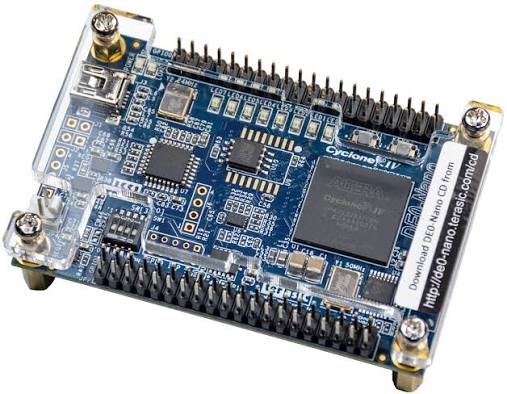
\includegraphics[width=\textwidth]{Figs/placa.jpg}
		%	\centering \textit{[Imagem da placa DE0-Nano]}
		\end{column}
	\end{columns}
\end{frame}


%----------------------------------------------------------------------------------------
\section{Referências bibliográficas}
%====================================================================================================

%\begin{frame}{Produção bibliográfica}
%	
%	
%	\begin{itemize}
%	\justifying
%	
%	\item CABRAL, FELIPE ; ANACONA-MOSQUERA, OSCAR ; SAMPAIO, RENATO C. ; TEODORO, GEORGE ; LLANOS, CARLOS H. ; JACOBI, RICARDO P. . Optimized execution of morphological reconstruction in large medical images on embedded devices. Journal of Real-Time Image Processing, v. 1, p. 1, 2020. 			
%	
%	\item ANACONA-MOSQUERA, OSCAR; SANTOS, CARLOS E. ; CABRAL, FELIPE R. G. ; SAMPAIO, RENATO C. ; TEODORO, GEORGE ; JACOBI, RICARDO P. ; LLANOS, CARLOS H. . Hardware-Based Fast Hybrid Morphological Reconstruction. IEEE Design \& Test, v. 1, p. 1-1, 2019. 
%	
%%	\item ANACONA-MOSQUERA, OSCAR; CABRAL, FELIPE R. G. ; SAMPAIO, RENATO C. ; TEODORO, GEORGE ; JACOBI, RICARDO P. ; LLANOS, CARLOS H. . Efficient Hardware Implementation of the Fast Hybrid Morphological Reconstruction Algorithm. In: 2018 31st Symposium on Integrated Circuits and Systems Design (SBCCI), 2018, Bento Gonçalves - RS. 2018 31st Symposium on Integrated Circuits and Systems Design (SBCCI), 2018. p. 1. 
%	
%%	\item ANACONA-MOSQUERA, OSCAR; TEODORO, GEORGE ; VINHAL, GUSTAVO ; JACOBI, RICARDO P. ; SAMPAIO, RENATO C. ; LLANOS, CARLOS H. . Efficient hardware implementation of morphological reconstruction based on sequential reconstruction algorithm. In: the 30th Symposium, 2017, Fortaleza. Proceedings of the 30th Symposium on Integrated Circuits and Systems Design Chip on the Sands - SBCCI '17. New York: ACM Press, 2017. p. 162. 
%	
%%	\item ANACONA-MOSQUERA, OSCAR; ARIAS-GARCIA, JANIER ; MUNOZ, DANIEL M. ; LLANOS, CARLOS H. . Efficient hardware implementation of the Richardson-Lucy Algorithm for restoring motion-blurred image on reconfigurable digital system. In: 2016 29th Symposium on Integrated Circuits and Systems Design (SBCCI), 2016, Belo Horizonte. 2016 29th Symposium on Integrated Circuits and Systems Design (SBCCI). p. 1. 
%	
%	\end{itemize}
%	
%\end{frame}
%----------------------------------------------------------------------------------------



\end{document}
